\section{Lecture 2}

\subsection{Style Guide}
We provide an informal style guide for writing mathematical proofs. 

\begin{center}
    \begin{tabular}{l|l|c}
     Goal & Knowledge & \shortstack[c]{Outermost\\symbol} \\
    \hline 
        \pbox{20cm}{Show for all $x$, $G(x)$. \\ Consider arbitrary $\hat{x}{}^1$.\\ Show $G(\hat{x})$}
      & \pbox{20cm}{We know for all $x$, $K(x)$ \\ In particular we know $K(\hat{t}){}^2$}
      & $\forall$ \\
    \hline 
        \pbox{20cm}{Show: exists $x$ s.t. $G(x)$. \\ We show $G(\hat{t}){}^2$}
      & \pbox{20cm}{We know exists $x$ s.t. $K(x)$ \\ Let $\hat{x}{}^1$ be s.t. $K(\hat{x})$}
      & $\exists$ \\
    \hline
        \pbox{20cm}{Show if $G_1$ then $G_2$ \\ Assume $G_1$\\ Show $G_2$}
      & \pbox{20cm}{We know if $K_1$ then $K_2$\\ To show $K_2$ it suffices to show $K_1$\\ Know $K_1$, Also know $K_2$}
      & $\Rightarrow$ \\
    \hline
        \pbox{20cm}{Show $G_1$ iff $G_2$ \\ 1. Show if $G_1$ then $G_2$\\ 2. Show if $G_2$ then $G_1$}
      & \pbox{20cm}{We know $K_1$ iff $K_2$\\ In particular we know if $K_1$ then $K_2$\\ and if $K_2$ then $K_1$}
      & $\iff$ \\
    \hline
        \pbox{20cm}{Show $G_1$ and $G_2$\\ 1. Show $G_1$, \textbf{and}\\ 2. Show $G_2$}
      & \pbox{20cm}{Know $K_1$ and $K_2$\\ Also Know $K_1$ \\ Also Know $K_2$}
      & $\wedge$ \\
    \hline
        \pbox{20cm}{Show $G_1$ or $G_2$\\ Either, assume $\neg G_1$, show $G_2$, \textbf{or}\\ Assume $\neg G_2$, show $G_1$}
      & \pbox{20cm}{We know $K_1$ or $K_2$. Show $G$.\\ case 1: Assume $K_1$, Show $G$\\ case 2: Assume $K_2$, Show $G$ \\ Case split $\uparrow$}
      & $\vee$ \\
    \hline
     \multicolumn{2}{c|}{\pbox{20cm}{Move Negation Inside, as far as possible}} &  $\neg$ \\ 
    \hline
     \multicolumn{3}{c}{$\rule{0pt}{1.5em} {}^1$ where $\hat{x}$ is a new constant.\hspace{2em} ${}^2$ where $\hat{t}$ is any constant expression}
\end{tabular}
\end{center}


\subsection{Lattices and Fixpoints}
We define relations and their properties. 

\begin{definition}[Relation]
A binary \emph{relation} $R$ on a set $A$ is a subset $R \subseteq A\times A$.
The relations $R$ is:
\begin{itemize}
    \item \emph{reflexive} if for all $x$ in $A$, we have $R(x,x)$.
    \item \emph{anti-symmetric} if for all $x$ and $y$ in $A$, if $R(x,y)$ and $R(y,x)$ then $x=y$.
    \item \emph{transitive} if for all $x,y$ and $z$ in $A$, if $R(x,y)$ and $R(y,z)$ then $R(x,z)$.
    \item a \emph{partial order} if $R$ is reflexive, anti-symmetric and transitive.
\end{itemize}
\end{definition}

\begin{definition}[poset]
     A \emph{poset} $(A,\sqsubseteq)$ is a set $A$ and a partial order $\sqsubseteq$ on $A$.
\end{definition}


\begin{example}
    Let $\NN$ be the natural numbers. The pair $(\NN,\leq)$ is a poset.
\begin{center}
     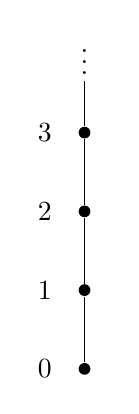
\begin{tikzpicture}[scale=1, every node/.style={circle, fill, inner sep=1.5pt}, 
    label distance=2mm]

    % Nodes
    \node[label=left:{$0$}] (0) at (0, 0) {};
    \node[label=left:{$1$}] (1) at (0 ,1) {};
    \node[label=left:{$2$}] (2) at (0, 2) {};
    \node[label=left:{$3$}] (3) at (0, 3) {};
   \node[draw=none, fill=none] (4) at (0,4) {$\vdots$};  % Dots to indicate continuation
   
    % Lines
    \draw (0) -- (1);
    \draw (1) -- (2);
    \draw (2) -- (3);
    \draw (3) -- (4);

\end{tikzpicture}
 \end{center}
\end{example}

% \begin{example}
   
   
%     \begin{figure}[h]
%         \centering
%         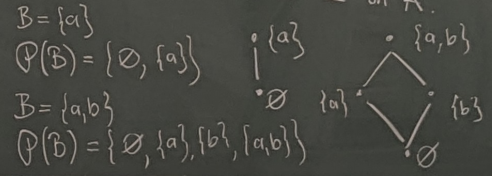
\includegraphics[width=0.7\linewidth]{images/poset.png}
%     \end{figure}
% \end{example}


\begin{example}
 For any set $B$ let $\power(B)$ be the powerset.
 The pair $(\power(B),\subseteq)$ is a poset. E.g., for $B\coloneqq \{a\}$ (left) and for $B \coloneqq \{a,b\}$ (right).
 \begin{center}
 
     \begin{tikzpicture}[scale=1, every node/.style={circle, fill, inner sep=1.5pt}, 
    label distance=2mm]

     \node[label=right:{$\emptyset$}] (0) at (-6,0 ) {};
    \node[label=right:{$\{a\}$}] (1) at (-6,2 ) {};
    % Nodes
    \node[label=right:{$\emptyset$}] (emptyset) at (0, 0) {};
    \node[label=left:{$\{a\}$}] (a) at (-1, 1) {};
    \node[label=right:{$\{b\}$}] (b) at (1, 1) {};
    \node[label=right:{$\{a,b\}$}] (ab) at (0, 2) {};
    
    % Lines
    \draw (0) -- (1);
    
    \draw (emptyset) -- (a);
    \draw (emptyset) -- (b);
    \draw (a) -- (ab);
    \draw (b) -- (ab);

\end{tikzpicture}
 \end{center}

\end{example}

\begin{definition}[Upper Bound]
    Let $(A,\sqsubseteq)$ be a poset. Then (i) $x$ in $A$ is an \emph{upper bound} of a subset $B$ of $A$ if for all $y$ in $B$, it holds that $y \sqsubseteq x$;
    (ii) $x$ is the \emph{least upper bound} (lub) of $B$ if $x$ is an upper bound of $B$ and for all upper bounds $y$ of $B$, we have $x \sqsubseteq y$. %We denote such $x$ by $\bigsqcup B$.
\end{definition}

\begin{definition}[Lower Bound]
    Let $(A,\sqsubseteq)$ be a poset. Then (i) $x$ in $A$ is a \emph{lower bound} of a subset $B$ of $A$ if for all $y$ in $B$, it holds that $x \sqsubseteq y$;
    (ii) $x$ is the \emph{greatest lower bound} (glb) of $B$ if $x$ is a lower bound of $B$ and for all lower bounds $y$ of $B$, we have $y \sqsubseteq x$. %We denote such $x$ by $\bigsqcap B$.
\end{definition}

\begin{example}
    Consider the poset $(\NN,\leq)$. Then for any $B \subseteq \NN$, if $B$ is finite, $\lub(B)$ is well-defined and equal to $\max(B)$. If $B$ is infinite, then $\lub(B)$ does not exist.
\end{example}

\begin{example}
   Consider the poset $(\NN \cup \{\infty\},\leq)$ where for all $x$ in $\NN$, it holds that $x \leq \infty$. Then for all $B \subseteq \NN$, $\lub(B)$ is well-defined.
\end{example}

\begin{example}
    Let $A$ be any set and consider the poset $(\power(A),\subseteq)$. For any subset $B$ of $\power(A)$, it holds that $\lub(B) = \bigcup B$ and $\glb(B) = \bigcap B$.
\end{example}

\begin{lemma}
  Let $(A,\sqsubseteq)$ be a poset. For all $x$, $y$ in $A$, and any subset $B$ of $A$, if $x$ and $y$ are lubs (glbs) of $B$, then $x = y$.
\end{lemma}

\begin{proof}
    Consider arbitrary $\hat{x}, \hat{y} \in A$ and $\hat B \subseteq A$. Assume $\hat x$ is a lub of $\hat B$
    and $\hat y$ is a lub of $\hat B$. We know:
    \begin{enumerate}
        \item[(i)] for all $z \in B$, $z \sqsubseteq \hat{x}$,
        \item[(ii)] for all $z \in B$, $z \sqsubseteq \hat{y}$,
        \item[(iii)] for all $z \in A$, if $z$ is an upper bound of $B$ then
        $\hat x \sqsubseteq z$ and
        \item[(iv)]for all $z \in A$, if $z$ is an upper bound of $B$ then $\hat
        y \sqsubseteq z$.
    \end{enumerate}
    From (ii) we know that $\hat{y}$ is an upper bound, and therefore, by (iii), $\hat{x} \sqsubseteq \hat{y}$. Symmetrically, by (i) and (iv) we get $\hat{y} \sqsubseteq \hat{x}$. By antisymmetry, $x = y$.
\end{proof}

Given that the \emph{least upper bound} and the \emph{greatest lower bound} are unique (if they exist), for any set $A$ and $B \subseteq A$, we write $\bigsqcup B$ to denote $\lub(B)$ and $\bigsqcap B$ to denote $\glb(B)$.

\begin{definition}[Lattice]
    A poset $(A,\sqsubseteq)$ is a \emph{lattice} if for all $x$, $y$ in $A$, the lub $\bigsqcup \{x,y\}$ ($x \sqcup y$, join) and the glb $\bigsqcap \{x,y\}$ ($x \sqcap y$, meet) exist.
\end{definition}

\begin{definition}[Complete Lattice]
    A poset $(A,\sqsubseteq)$ is a \emph{complete lattice} if for all $B \subseteq A$, the lub $\bigsqcup B$ and glb $\bigsqcap B$ exist.
\end{definition}

\begin{example}
    Let $(A,\sqsubseteq)$ be a complete-lattice. Then: $\bigsqcup A = \top$, $\bigsqcap A = \bot$, $\bigsqcup \varnothing = \bot$, and $\bigsqcap \varnothing = \top$. $\top$ and $\bot$ are called top and bottom, respectively.
\end{example}

\begin{definition}[Monotone Function]
Let $(A, \sqsubseteq)$ be a poset. A function $F: A \to A$ is \emph{monotone} if for all $x$, $y$ in $A$, if $x \sqsubseteq y$ then $F(x) \sqsubseteq F(y)$.
\end{definition}

\begin{definition}
Let $(A, \sqsubseteq)$ be a poset and $F: A \to A$. An element $x$ in $A$ is,
\begin{enumerate}
  \item a \emph{prefixpoint} of $F$ if $x \sqsubseteq F(x)$,
  \item a \emph{postfixpoint} of $F$ if $F(x) \sqsubseteq x$.
\end{enumerate}
\end{definition}

% TODO
\begin{definition}[Fixpoint]
Let $(A, \sqsubseteq)$ be a poset and $F: A \to A$. An element $x$ in $A$ is a \emph{fixpoint} of $F$ if it is both a \emph{pre-} and \emph{postfixpoint} of $F$.
\end{definition}

\begin{theorem}[Knaster-Tarski]
\label{thrm:knaster}
    Let $(A,\sqsubseteq)$ be a complete lattice and let $F$ be a monotone function on $A$.
    Further, let $\hat{y} = \bigsqcup \{x \mid x \sqsubseteq F(x)\}$ and $\hat{z} = \bigsqcap\{x \mid F(x) \sqsubseteq x\}$.
    It holds, that:
    \begin{enumerate}
      \item $\hat{y}$ and $\hat{z}$ are fixpoints of $F$,
      \item for all fixpoints $x$ of $F$, $\hat{z} \sqsubseteq x \sqsubseteq \hat{y}$
    \end{enumerate}
\end{theorem}

{\flushleft We write $\lfp(F) = \bigsqcap\{x \mid F(x)\sqsubseteq x\}$ and $\gfp(F) = \bigsqcup\{x \mid x \sqsubseteq F(x)\}$, to denote the least fixpoint and the greatest fixpoint, respectively.}

\begin{exercise}
        Prove the Knaster Tarski Theorem (Theorem \ref{thrm:knaster}).
\end{exercise}


